%%%%%%%%%%%%%%%%%%%%%%%%%%%%%%%%%%%%%%%%%
% Journal Article
% LaTeX Template
% Version 1.4 (15/5/16)
%
% This template has been downloaded from:
% http://www.LaTeXTemplates.com
%
% Original author:
% Frits Wenneker (http://www.howtotex.com) with extensive modifications by
% Vel (vel@LaTeXTemplates.com)
%
% License:
% CC BY-NC-SA 3.0 (http://creativecommons.org/licenses/by-nc-sa/3.0/)
%
%%%%%%%%%%%%%%%%%%%%%%%%%%%%%%%%%%%%%%%%%

%----------------------------------------------------------------------------------------
%	PACKAGES AND OTHER DOCUMENT CONFIGURATIONS
%----------------------------------------------------------------------------------------

\documentclass[twoside,twocolumn,10pt]{article}

\usepackage[T1]{fontenc} % Use 8-bit encoding that has 256 glyphs
\usepackage{microtype} % Slightly tweak font spacing for aesthetics

\usepackage[hmarginratio=1:1,top=32mm, left=20mm, right=20mm,columnsep=20pt]{geometry} % Document margins
\usepackage[hang, small,labelfont=bf,up,textfont=it,up]{caption} % Custom captions under/above floats in tables or figures
\usepackage{booktabs} % Horizontal rules in tables

\usepackage{enumitem} % Customized lists
\setlist[itemize]{noitemsep} % Make itemize lists more compact

\usepackage{abstract} % Allows abstract customization
\renewcommand{\abstractnamefont}{\normalfont\bfseries} % Set the "Abstract" text to bold
\renewcommand{\abstracttextfont}{\normalfont\small\itshape} % Set the abstract itself to small italic text

\usepackage{titlesec} % Allows customization of titles
\renewcommand\thesection{\Roman{section}} % Roman numerals for the sections
\renewcommand\thesubsection{\roman{subsection}} % roman numerals for subsections
\titleformat{\section}[block]{\large\scshape\centering}{\thesection.}{1em}{} % Change the look of the section titles
\titleformat{\subsection}[block]{\large}{\thesubsection.}{1em}{} % Change the look of the section titles

\usepackage{fancyhdr} % Headers and footers
\pagestyle{fancy} % All pages have headers and footers
\fancyhead{} % Blank out the default header
\fancyfoot{} % Blank out the default footer
%\fancyhead[C]{Progetto di Ingegneria Informatica $\bullet$ Post-Quantum Cryptography} % Custom header text
\fancyfoot[RO,LE]{\thepage} % Custom footer text

\usepackage{titling} % Customizing the title section
\usepackage{hyperref} % For hyperlinks in the PDF
\usepackage{amsmath}
\usepackage{dsfont} % For \mathds commands
\usepackage{graphicx}
\usepackage{mathtools}
\usepackage{booktabs}
\usepackage{pgfplots}
\usepackage{mathtools}
\usepackage{amssymb}

\DeclarePairedDelimiter\ceil{\lceil}{\rceil}
\DeclarePairedDelimiter\floor{\lfloor}{\rfloor}

\usepackage[ruled,vlined,linesnumbered]{algorithm2e}
%----------------------------------------------------------------------------------------
%	TITLE SECTION
%----------------------------------------------------------------------------------------

\setlength{\droptitle}{-4\baselineskip} % Move the title up

\bibliographystyle{ieeetr}



\pretitle{\begin{center}\Huge\bfseries} % Article title formatting
\posttitle{\end{center}} % Article title closing formatting
\title{Protecting HQC decryption from side-channel differential power analysis} % Article title
\author{%
\textsc{Domenico Cacace -- 977835}}
\date{} % Leave empty to omit a date
\renewcommand{\maketitlehookd}{%
\begin{abstract}
This work describes a masking-based side channel resistent implementation of HQC, a third round alternative candidate for the NIST Post-Quantum Cryptography competition.
The presented implementation is then tested on an ARM Cortex-M4 processor; the test results show a significant decrease in terms of leaked information, while keeping the overhead factor due to the masking below 2.
\end{abstract}
}

%----------------------------------------------------------------------------------------

\begin{document}

% Print the title
\maketitle

\section{Introduction}
The security of current public key cryptosystems is based on the \textit{hardness} of some mathematical problems, such as large integer factorization or discrete logarithm extraction; however, such problems could become tractable, thanks to the Shor's algorithm, with the aid of a large scale quantum computer.
For this reason in 2017 the National Institute of Standards and Technology (NIST) started a procedure for the standardization of cryptographic primitives able to withstand such kind of attacks.

Many proposals, such as Hamming Quasi-Cyclic (HQC), are based on \textit{hard} problems of coding theory; even though, the implementation of the cryptosystem can be vulerable to side channel attacks, that can exploit the information leaked by phisically measurable channels (\textit{e.g.} EM fields, power consumption).

In this paper we make a brief recap of the basics of coding theory and an overview of the cryptosystem. We present a masking scheme suitable for HQC, then implement and benchmark this scheme on an ARM Cortex-M4 microprocessor. 

\section{Preliminaries}\label{preliminaries}
\subsection*{\textbf{General definitions}}
We denote with $\mathds{F}_{2}$ the binary finite field, with $\mathds{Z}$ the integer ring and with ${\mathcal{V} = \mathds{F}_{2}^{n}}$ a vector space of dimension $n$ over $\mathds{F}_2$ for some positive integer $n \in \mathds{Z}$; 
elements of $\mathcal{V}$ can be interchangeably considered as row vectors or polynomials in ${\mathcal{R} = \mathds{F}_{2}[X]/(X^n-1)}$.
Additionally, we denote by $\omega(\cdot)$ the Hamming weight of a vector \textit{i.e.} the number of its non-zero coordinates.

Let ${\mathbf{v} = (v_0, \cdots, v_{n-1}) \in \mathcal{V}}$. The circulant matrix induced by $v$ is defined as
\begin{equation*}
    \textbf{rot}(\mathbf{v}) = 
    \begin{pmatrix}
        v_0 & v_{n-1} & \cdots & v_1 \\
        v_1 & v_0 & \cdots & v_2 \\
        \vdots & \vdots & \ddots & \vdots \\
        v_{n-1} & v_{n-2} & \cdots & v_0 \\
    \end{pmatrix}
    \in \mathds{F}_{2}^{n\times n}
\end{equation*}

\subsection*{\textbf{Coding theory}\cite{macwilliams1977theory}}
A linear code $\mathcal{C}$ of length $n$ and dimension $k$ (denoted as $[n, k]$) is a subspace of $\mathcal{V}$ of dimension $k$. Elements of $\mathcal{C}$ are called \textit{codewords}.\\

We say that ${\textbf{G} \in \mathds{F}^{k\times n}_{2}}$ is a generator matrix for the code $\mathcal{C}$ if
\begin{equation*}
    \mathcal{C} = \lbrace \textbf{mG}, \text{for } \textbf{m} \in \mathds{F}_2^k \rbrace
\end{equation*}

Given a $[n, k]$ code $\mathcal{C}$, we say that the matrix ${\mathbf{H}\in\mathds{F}_2^{(n-k)\times n}}$ is a Parity-Check matrix for $\mathcal{C}$ if it is a generator matrix of the dual code $\mathcal{C}^{\bot}$ or, in other words, 
\begin{equation*}
\mathcal{C} = \lbrace \mathbf{v} \in \mathds{F}_2^n \text{ such that } \mathbf{Hv^{\top}} = \mathbf{0} \rbrace
\end{equation*}

Given ${\mathbf{H} \in \mathds{F}_2^{(n-k)\times n}}$ a parity matrix for some code $\mathcal{C}$ and a word ${\mathbf{v} \in \mathds{F}_2^n}$, we call $\mathbf{Hv}^{\top}$ the syndrome of $\mathbf{v}$. From the definition of parity-check matrix, it holds that:
\begin{equation*}
    \mathbf{v} \in \mathcal{C} \iff \mathbf{Hv}^{\top} = \mathbf{0}
\end{equation*}

Given a linear code $\mathcal{C}$ over $\mathcal{V}$ and $\omega$ a norm on $\mathcal{V}$, we define the minimum distance of $\mathcal{C}$ as
\begin{equation*}
    d = \min_{\mathbf{u, v} \in \mathcal{C}, \mathbf{u}\neq \mathbf{v}} \omega(\mathbf{u} - \mathbf{v})
\end{equation*}
A code with minimum distance $d$ is capable of decoding an arbitrary pattern of up to $\delta = \lfloor \frac{d-1}{2}\rfloor$ errors; such a code is also denoted as $[n, k. d]$.\\

Consider a vector $\mathbf{c} = (\mathbf{c}_0, \cdots, \mathbf{c}_{s-1}) \in \mathds{F}_2^{sn}$ as $s$ successive $n$-uples; a $[sn, k, d]$ linear code $\mathcal{C}$ is said to be Quasi-Cyclic (QC) of order $s$ if, for any $\mathbf{c} = (\mathbf{c}_0, \cdots, \mathbf{c}_{s-1}) \in \mathcal{C}$, the vector obtained by applying a simultaneous circular shift to every block $\mathbf{c}_i$ is also a codeword.

\subsubsection*{Decoding}

When dealing with linear codes, the problem of decoding a vector stays the same when we use the syndrome of the vector, so we speak of Syndrome Decoding (SD).\\

For positive integers $n$, $k$ and $w$ the SD($n, k, w$) distribution \textit{chooses} $\mathbf{H} \xleftarrow{\mathdollar} \mathds{F}_2^{(n-k)\times n}$ and $\mathbf{x} \xleftarrow{\mathdollar} \mathds{F}_2^n$ such that $\omega(\mathbf{x}) = w$ and outputs the couple $(\mathbf{H}, \mathbf{Hx}^{\top})$.\\

On input $(\mathbf{H}, \mathbf{y}^{\top})$ from the SD Distribution, the Syndrome Decoding problem SD($n, k, w$) asks to find a vector $\mathbf{x}$ such that $\mathbf{Hx}^{\top} = \mathbf{y}^{\top}$ and $\omega(\mathbf{x}) = w$; for the Hamming distance this problem has been proven to be NP-complete~\cite{berlekamp1978inherent}.\\

The decisional version of the SDP requires to determine, given $(\mathbf{H}, \mathbf{y}^{\top}) \in \mathds{F}_2^{(n-k)\times n} \times \mathds{F}_2^{(n-k)}$, if $(\mathbf{H}, \mathbf{y}^{\top})$ comes from the SD($n, k, w$) or the uniform distribution over $\mathds{F}_2^{(n-k)\times n} \times \mathds{F}_2^{(n-k)}$; in other words, this is the problem of decoding random linear codes from random errors.



\section{Cryptosystem Overview}
 Hamming Quasi-Cyclic (HQC) is a cryptosystem running for standardization to NIST's competition in the category ``post-quantum public key encryption scheme''~\cite{melchor2018hamming}.
It is a code-based cryptosystem, and its security is based on the hardness of a variant of the Decisional SD Problem, reported in~\cite{aguilar2018efficient}.\\
In order to cope with the huge key sizes associated with code-based cryptosystems, HQC adopts Quasi-Cyclic (QC) codes~\cite{gaborit2005shorter}; there is no general complexity result for the decoding of QC codes, but this problem is considered hard by the community.\\

HQC consists of two schemes: a Public Key Encryption (PKE) and a Key Encapsulation/Data Encapsulation Mechanism (KEM/DEM).

\subsubsection*{\textbf{\textsf{HQC.PKE}}}
The PKE employs a decodable $[n, k]$ code $\mathcal{C}$ generated by $\mathbf{G}\in \mathds{F}_2^{k\times n}$, which can correct at most $\delta$ errors with the $\mathcal{C}$.\textsf{Decode}($\cdot$) algorithm, and a random double-circulant $[2n, n]$ code with parity-check matrix $(\mathbf{1}, \mathbf{h})$; the algorithms that constitute this scheme are the following:

\begin{itemize}
  \item \textsf{Setup}(): generate and returns the parameters \textsf{param}=($n, k, \delta, w, w_{\mathbf{r}}, w_{\mathbf{e}}$).
  \item \textsf{KeyGen}(\textsf{param}): sample a random vector $\mathbf{h}$ for the parity-check matrix, the generator matrix $\mathbf{G}$ (which is public), the private key \textsf{pk} as a couple of random vectors $(\mathbf{x}, \mathbf{y}) \in \mathcal{R}^2$ both oh Hamming weight equal to $w$, then set the public key \textsf{pk} = ($\mathbf{h}$, $\mathbf{s} \leftarrow \mathbf{x}+\mathbf{h\cdot y}$); return the keys (\textsf{pk}, \textsf{sk}).
  \item \textsf{Encrypt}(\textsf{pk}, $\mathbf{m}$): generate the random vectors\\ $\mathbf{e} \in \mathcal{R}$, $(\mathbf{r}_1, \mathbf{r}_2) \in \mathcal{R}^2$ such that $\omega(\mathbf{e}) = w_{\mathbf{e}}$ and $\omega(\mathbf{r}_1) = \omega(\mathbf{r}_2) = w_{\mathbf{r}}$, then calculate the ciphertext as $\mathbf{c} = (\mathbf{u}, \mathbf{v}) = (\mathbf{r}_1 + \mathbf{h}\cdot\mathbf{r}_2, \mathbf{mG} + \mathbf{s}\cdot\mathbf{r}_2 + \mathbf{e})$
  \item \textsf{Decrypt}(\textsf{sk}, $\mathbf{c}$): return $\mathcal{C}$.\textsf{Decode}($\mathbf{v} - \mathbf{u\cdot y}$)
\end{itemize}
 
Although \textsf{sk} is composed of two vectors, $\mathbf{x}$ is only used to compute part of \textsf{pk} and it is not employed in the decryption phase.

\subsubsection*{\textbf{\textsf{HQC.KEM}}}
The KEM is built upon an instance of \textsf{HQC.PKE} $\mathcal{E}$ and three hash functions $\mathcal{G}, \mathcal{H}, \mathcal{K}$, with $\mathcal{G} \neq \mathcal{H}$.
The setup and key generation algorithms are the same of the PKE, with the exception that $k$ now is the lenght of the shared key.
\begin{itemize}
  \item \textsf{Encaps}(\textsf{pk}): generate a random $\mathbf{m} \in \mathds{F}_2^k$ to derive the randomness $\theta \leftarrow \mathcal{G}(\mathbf{m})$; 
  generate the ciphertext $\mathbf{c} \leftarrow \mathcal{E}.\textsf{Encrypt}(\textsf{pk}, \mathbf{m}, \theta)$, derive the symmetric key $K \leftarrow \mathcal{K}(\mathbf{m}, \mathbf{c})$
    and send $(\mathbf{c}, \mathbf{d} = \mathcal{H}(\mathbf{m}))$
  \item \textsf{Decaps}(\textsf{sk}, $\mathbf{c}$, $\mathbf{d}$): decrypt $\mathbf{\bar{m}} \leftarrow \mathcal{E}.\textsf{Decrypt}(\textsf{sk}, \mathbf{c})$, compute $\bar{\theta} \leftarrow \mathcal{G}(\mathbf{\bar{m}})$ and use them to calculate 
  $\mathbf{\bar{c}} \leftarrow \mathcal{E}(\textsf{pk}, \mathbf{\bar{m}}, \bar{\theta})$: at this point if both $\mathbf{c} = \mathbf{\bar{c}}$ and $\mathbf{d} = \mathcal{H}(\mathbf{\bar{m}})$
    we can derive the shared key $K \leftarrow \mathcal{K}(\mathbf{\bar{m}}, \mathbf{\bar{c}})$. 
\end{itemize}

\section{Masking}

\begin{frame}
    \sectionpage
\end{frame}

\begin{frame}{Side Channel Attacks}
    Implementations of theoretically secure cryptosystems may \textit{leak} some information, allowing an 
    attacker to extract secret data.
    \begin{block}{Side Channel Vulnerabilities}
        Side channel attacks take use of different leakage sources, such as:
        \begin{itemize}
            \item Execution time
            \item Power consumption
            \item Electromagnetic radiation
            \item Differential faults
        \end{itemize}
    \end{block}
\end{frame}

\begin{frame}{Power Analysis}
    \begin{block}{Simple Power Analysis}
        Analyze the electrical current drawn by the device over time: different operations may have different power consumption.
    \end{block}
    \begin{block}{Differential Power Analysis}
        Statistically analyze the power consumption of the device over different executions: detect biases between, for example, a known secret key and a unknown one.
    \end{block}
\end{frame}

\begin{frame}{Power Analysis}
    \begin{figure}
        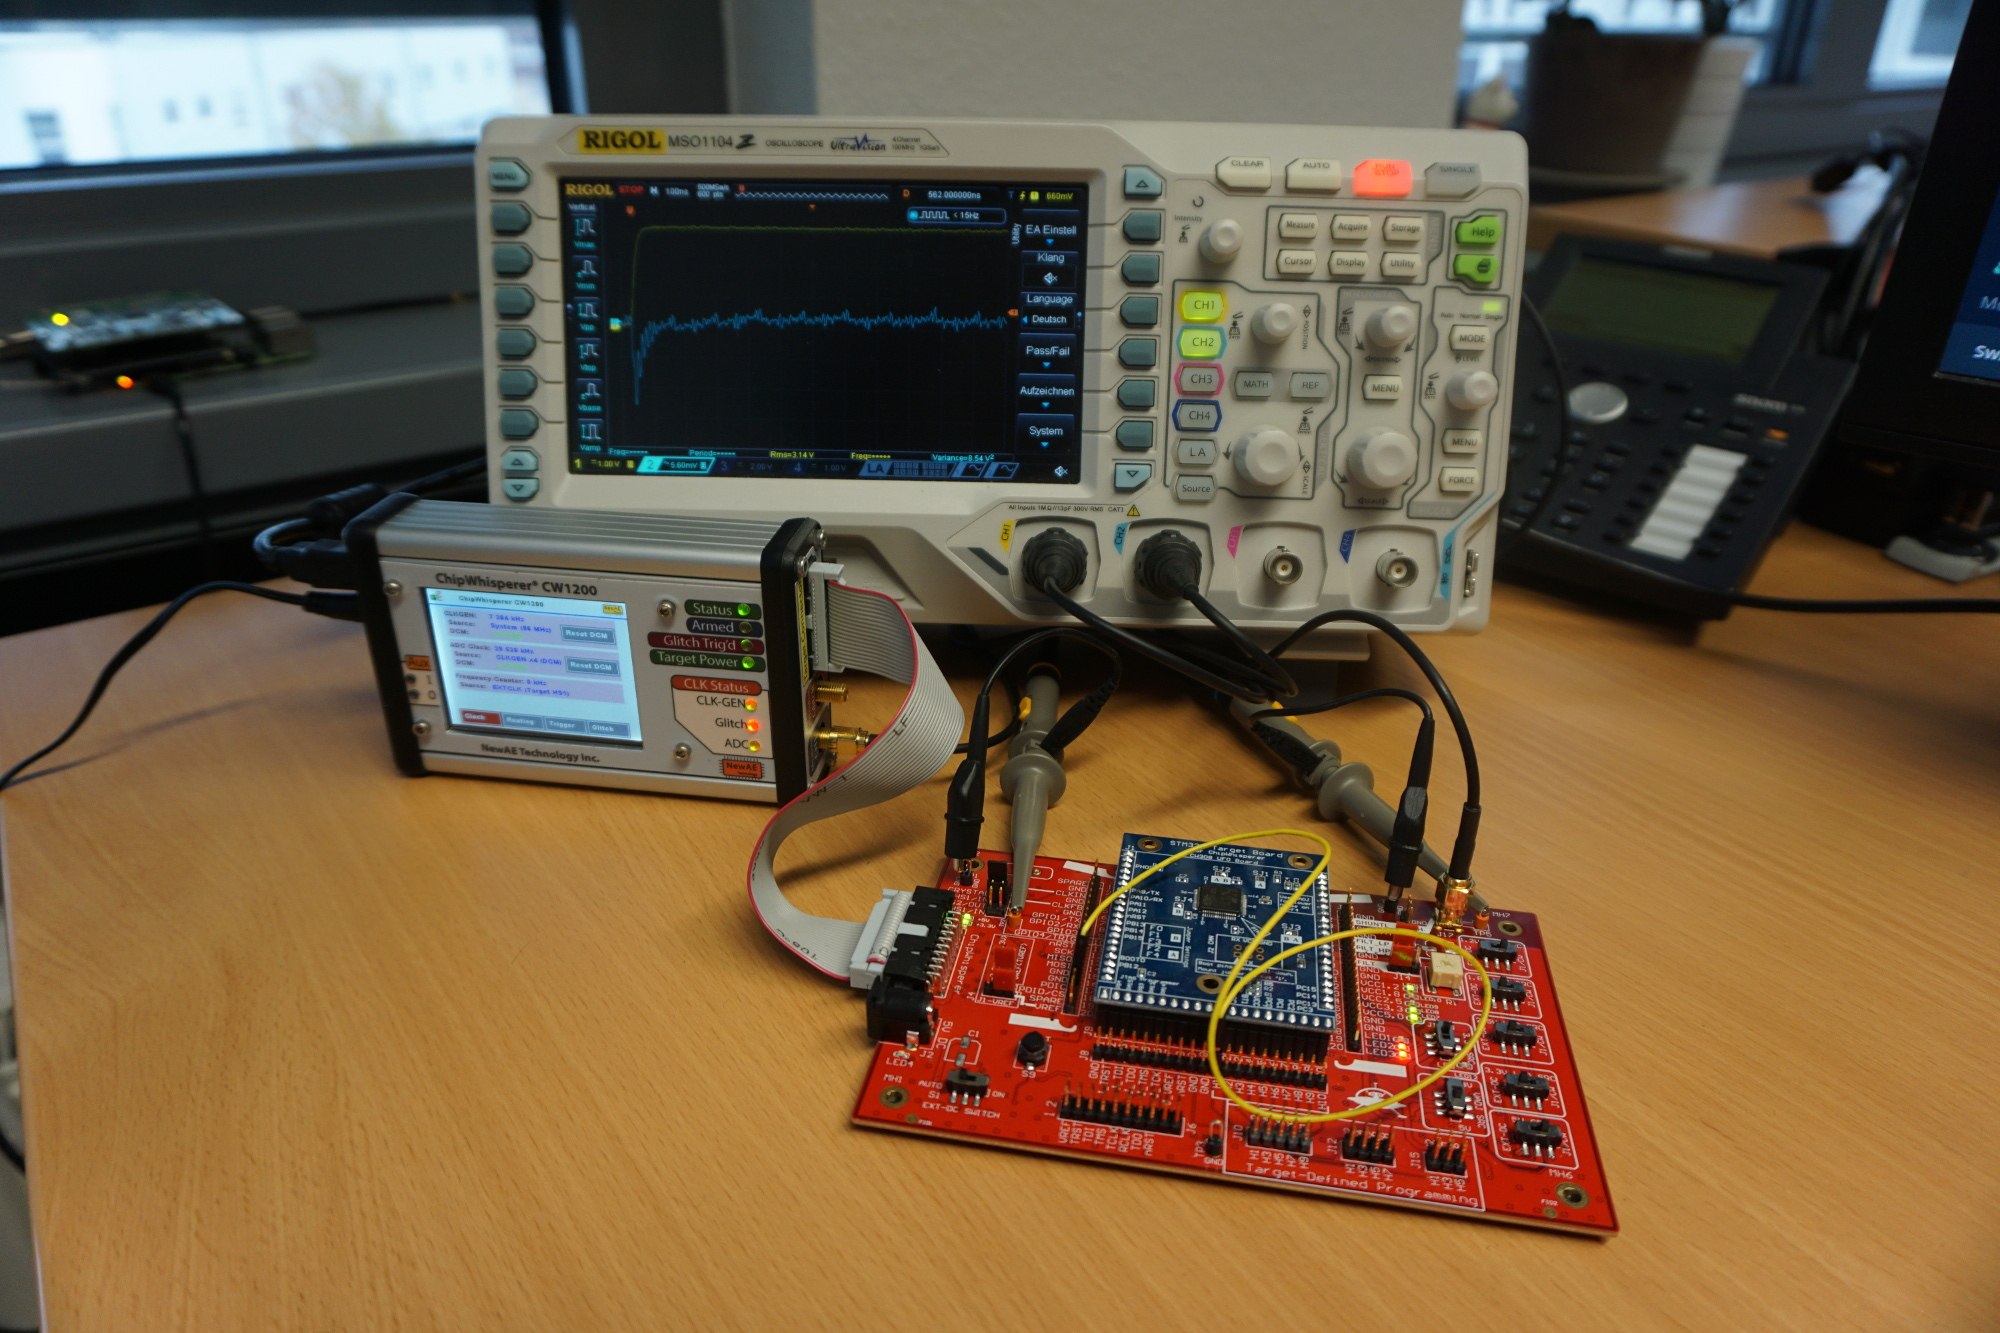
\includegraphics[scale=0.6]{images/chipwhisperer_with_target_and_oscilloscope.jpg}
        \caption{ChipWhisperer}
        % \footnote{https://www.schutzwerk.com/en/43/posts/poweranalysis\_1/}
    \end{figure}
    
\end{frame}

\begin{frame}{Countermeasures to Power Analysis}
    Power analysis attacks are usually passive, so they cannot be detected by the device.
    \begin{block}{}
        To mitigate the effectiveness of these attacks, it is possible to:
        \begin{itemize}
            \item \textbf{SPA}: avoid branches with conditions that depend on secret data
            \item \textbf{DPA}: \textit{mask} the secret data when performing operations on them
        \end{itemize}
    \end{block}
    \begin{block}{Masking}
        Given a secret $x$, we can split it into $d$ \textit{shares} in such a way that
        \begin{equation*}
            x = x_0 \odot x_1 \cdots \odot x_{d-1}
        \end{equation*}
        for some operation $\odot$ (e.g. XOR in binary fields).
    \end{block}
\end{frame}

\begin{frame}{Securing AND gates}
    \begin{block}{Probing Model~\cite{ishai2003private}}
        Given an algorithm that operates on data split among $d$ shares, we say that the algorithm is 
        secure against a $(d-1)$-th order probing attack if, on input $x = (x_1, \cdots, x_d)$, it admits no
        tuple of $d-1$ (or less) shares that depends on $x$
    \end{block}
    \begin{block}{Ishai-Sahai-Wagner’s Scheme}
        Let $x = (x_1, \cdots, x_d), y = (y_1, \cdots, y_d)$ binary variables: to securely compute $x \wedge y$ at order $\lfloor d/2 \rfloor$:
        \begin{itemize}
            \item Pick a random bit $r_{i, j}$
            \item Compute $r_{j, i} = (r_{i, j} + (x_i \wedge y_j)) + (x_j \wedge y_i)$
            \item Compute $c_i = (x_i \wedge y_j) + \sum_{j \neq i} r_{i, j}$ 
        \end{itemize}
    \end{block}
\end{frame}

\begin{frame}{Securing multiplications}
    The ISW scheme can be extended from $\mathds{F}_2$ to $\mathds{F}_2^{n}$, increasing its security to $d$-th order attacks
    \begin{block}{Rivain-Prouff's Scheme}
        Let $a = (a_1, \cdots, a_d), b = (b_1, \cdots, b_d)$, with $ a_i, b_i \in \mathds{F}_2^n$
        \begin{itemize}
            \item Calculate $c_i \leftarrow a_i\cdot b_i$ for each share
        \end{itemize}
        For $i$ from 1 to $d$ and $j$ from $i+1$ to $d$:
        \begin{itemize}
            \item Extract a random value $s \xleftarrow{\$} \mathds{F}_2^n$
            \item Calculate $s^{'} \leftarrow (s + (a_i \cdot b_j)) + (a_j \cdot b_i)$
            \item Calculate $c_i \leftarrow c_i + s$ and  $c_j \leftarrow c_j + s^{'}$ 
        \end{itemize}
        The sum of the shares $(c_1, \cdots, c_d)$ yields the product $a\cdot b$
    \end{block}
\end{frame}
\section{Implementation}
As a starting point, we take the third version of the reference implementation\footnote{\href{https://pqc-hqc.org/download.php?file=hqc-reference-implementation\_2021-06-06.zip}{https://pqc-hqc.org/download.php?file=hqc-reference-implementation\_2021-06-06.zip}}; this is a self-contained C implementation that can be ported on virtually any architecture as-is.

\subsection*{\textbf{Target}}
Our target architecture is \texttt{ARMv7E}: in particular, our tests are run on the STM F401-RE board mounting a Cortex\textsuperscript{\textregistered} M4 processor. This particular board is equipped with 512KB of flash memory and 96KB of RAM: due to this characteristics and the large memory footprint of the cryptosystem, we were able to run HQC only at security level 1 (corresponding to 128 bits of security).
In order to interact with the system we employ the Hardware Abstraction Layer (HAL) drivers, generated by STM32CubeMX specifically for our configuration. We use the drivers to notify when the encryption process is taking place through the LED on the board and to allow communications over the USB debug interface, redirecting in the \texttt{syscalls.c} file the standard output to the debug bridge for logging purposes.
To generate random variables required we employ the \texttt{seedexpander} function from SHAKE256~\cite{dworkin2015sha}.

\subsubsection*{\textbf{Objects representations}}
Elements of the various binary fields are represented as arrays. For randomly generated values, we employ the \texttt{seedexpander} function on a 40B seed.\\
The secret key \textsf{sk} = $(\mathbf{x}, \mathbf{y})$ is generated by $\mathbf{seed1}$, while the parity matrix $\mathbf{h}$ of the public key \textsf{pk}=$(\mathbf{h}, \mathbf{s})$ is generated by $\mathbf{seed2}$; the same principle applies for the random masks employed in the \texttt{safe\_mul} function. These values are sampled uniformly from the respective fields, with a given Hamming weight.\\
In all the multiplications, one of the operands is always a sparse polynomial: these polynomials are represented with a position vector of $\omega$ coordinates, containing the orders of the nonzero coefficients.

\subsubsection*{\textbf{Multiplication and masking}}
The multiplication over $\mathds{F}_2[X]/(X^n-1)$ is implemented with a slight variation of the scoolbook multiplication algorithm, since the sparsity of one of the operands yields a lower computational complexity than other methods.
This approach leaks information about the operands, which should remain secret: to overcome this problem we implemented a first-order masked multiplication scheme.\\

The dense ($a$) and sparse ($b$) polynomials are split in two halves, which are then combined accordingly to the ISW scheme; the \texttt{add} and \texttt{mult} function are an abstraction of the instructions that perform the addition and multiplication.

\begin{algorithm}
    \SetAlgoLined
    \SetKwFunction{secure_mult}{secure_mult}
    \KwIn{$a = (a_0a_1) \in \mathds{F}_2^n$ dense polynomial, $b = (b_0b_1)$ sparse polynomial, $\omega(b) = w$}
    \KwOut{$res, mask$ such that $res\oplus mask = a\cdot b$}
    \KwData{$temp_1, temp_2 \in \mathds{F}_2^n$}
    \SetKwProg{Fn}{function}{:}{}
    \BlankLine
    \BlankLine

    $mask \xleftarrow{\mathdollar_w} \mathds{F}_2^n$\\

    $temp_1 \leftarrow \texttt{mult}(a_1, b_0)$\\
    $temp_2 \leftarrow \texttt{mult}(a_0, b_1$)\\

    $res \leftarrow \texttt{add}(mask, temp_1)$\\
    $res \leftarrow \texttt{add}(res, temp_2)$\\

    $temp_1 \leftarrow \texttt{mult}(a_1, b_1)$\\
    $temp_2 \leftarrow \texttt{mult}(a_0, b_0$)\\

    $res \leftarrow \texttt{add}(res, temp_2)$\\
    $mask \leftarrow \texttt{add}(mask, temp_1)$\\

    \Return$res$, $mask$    
    \caption{First-order masked multiplication, 2 shares}
\end{algorithm}

We then generalized the masking procedure any number of by creating a small code generator to unroll the loops and reduce the execution time. 
We implemented and tested the masking procedure for $d \in \lbrace 2, 3, 4\rbrace$, as the number of operations grows with $\mathcal{O}(d^2)$.
\section{Results}
\begin{frame}
    \sectionpage
\end{frame}

\begin{frame}{Execution time}
    \begin{figure}
        \centering
        \begin{tikzpicture}[scale=0.9]
            \pgfplotsset{every axis/.append style={semithick}, legend style={at={(0,1)},anchor=north west, nodes={scale=0.6, transform shape}}}
    
        \begin{axis}[
            xlabel=Number of shares,ylabel=Clock cycles, grid=major,     x tick label style={
                /pgf/number format/.cd,
                precision=1,
            }]
    
        \addplot coordinates{
            (1, 2826067.47)
            (2, 3643555.40)
            (3, 4026514.86)
            (4, 4470225.81)
    
        };
        \addlegendentry{Encapsulation}
    
        \addplot coordinates{
            (1, 4445614.60)
            (2, 6070401.90)
            (3, 6819468.72)
            (4, 7680073.11)
    
        };
        \addlegendentry{Decapsulation}
    
        \addplot coordinates{
            (1, 1983894.79)
            (2, 2797433.27)
            (3, 3195107.26)
            (4, 3632298.13)
    
        };
        \addlegendentry{Encryption}
    
        \addplot coordinates{
            (1, 1584503.47)
            (2, 2405541.52)
            (3, 2770976.91)
            (4, 3193077.76)
    
        };
        \addlegendentry{Decryption}
    
        \addplot coordinates{
            (1, 624965.27)
            (2, 858842.66)
            (3, 1216993.20)
            (4, 1627512.25)
    
        };
        \addlegendentry{Multiplication}
        \end{axis}%
    \end{tikzpicture}%
    \end{figure}
\end{frame}

\begin{frame}{Execution Time}
    \begin{block}{Execution time (milliseconds)}
        \begin{table}
            \begin{tabular}{llllll}
                \# & encaps & decaps & enc & dec & mul \\ \hline
                1 & 201.86 & 317.54 & 141.71 & 113.18 & 44.64 \\
                2 & 260.25 & 433.60 & 199.82 & 171.82 & 61.35 \\
                3 & 287.61 & 487.10 & 228.22 & 197.93 & 86.93 \\
                4 & 319.30 & 548.58 & 259.45 & 228.08 & 116.25             
            \end{tabular}
        \end{table}
    \end{block}
    \begin{block}{Percentual performance decrease}
        \begin{table}
            \begin{tabular}{llllll}
                \# & encaps & decaps & enc & dec & mul \\ \hline
                2 & 28.92 & 36.55 & 41.00 & 51.81 & 37.42 \\
                3 & 42.48 & 53.40 & 61.05 & 74.88 & 94.73 \\
                4 & 58.18 & 72.76 & 83.09 & 101.51 & 160.41
            \end{tabular}
        \end{table}
    \end{block}
\end{frame}

\begin{frame}{Constant-time execution}
    \begin{block}{Welch's t-test}
        Given two statistical populations $X_1$ and $X_2$ of $N_1$ and $N_2$ samples respectively:
        \begin{equation*}
            t = \frac{\bar{X_1} - \bar{X_2}}{\sqrt{\frac{s_{X_1}^2}{N_1} + \frac{s_{X_2}^2}{N_2}}}
        \end{equation*}\\
    Can be used to verify that the means of the distributions are equal (null hypothesis).\\
    Setting the confidence to 99.999\%, we accept $H_0$ for $|t| \leq 4.5$
    \end{block}
\end{frame}

\begin{frame}{Constant-time execution}
    \begin{block}{Test Vector Leakage Assessment}
        Based on the Welch's t-test, defines the two groups as:
        \begin{itemize}
            \item Random: use different inputs for each computation
            \item Fixed: use the same inputs for all computations
        \end{itemize}
        In case of random data (\textit{e.g.} masks), these are always generated randomly.
    \end{block}
\end{frame}

\begin{frame}{Constant-time execution}
    \begin{block}{Welch's t}
        \begin{table}
            \begin{tabular}{llllll}
                \# & encaps & decaps & enc & dec & mul \\ \hline
                1 & 0.93666 & 4.56649 & 25.66178 & 10.26449 & 30.09420 \\
                2 & 6.00482 & 3.35650 & 4.62100 & 5.96089 & 4.96460 \\
                3 & 0.28901 & 1.69393 & 1.59911 & 5.88290 & 3.50812 \\
                4 & 0.12693 & NA\footnote{Not enough memory} & 3.30161 & 4.01299 & 0.21834
            \end{tabular}
        \end{table}        
    \end{block}
\end{frame}


\bibliography{refs}


\end{document}

